\documentclass{bxjsarticle}
\usepackage[utf8]{inputenc}

\usepackage{threeparttable}
\usepackage{float}
\usepackage{hyperref}
\usepackage{booktabs}
\usepackage[dvipdfmx]{graphicx}

\title{経済成長は格差を解消するか}
\author{小川創}
\date{December 2022}

\begin{document}

\maketitle
\begin{abstract}
    「国民の所得格差は、経済成長によって解消される」というクズネッツ曲線の仮説は正しいのか、日本とアメリカのデータを使って検証した。分析には、時系列データに対して高い汎用性のある状態空間モデルを用い、パラメータの分布はMCMCサンプルによって求めた。分析によって、国の経済成長は国民の所得格差には影響を与えない可能性が高いという結果が得られた。
\end{abstract}

\newpage


\section{はじめに}
\subsection{背景}
 経済成長の所得格差への影響について、経済成長の初期段階においては所得格差が拡大するが、ある程度経済成長が進展すると、所得格差は縮小していくという仮説がある。しかし、この仮説の理論的背景は、経済成長の初期段階で国の産業の比重が農業部門から工業部門にシフトし、その後、低所得者への待遇が改善されるだろうというものである。
\subsection{問い}
 このレポートでは以下の問いについて検証する。
\begin{itemize}
    \item 現代にアメリカと日本において、クズネッツ曲線の仮説は正しいといえるか。
\end{itemize}
 クズネッツ曲線の仮説は所得格差が縮小する段階では、工業部門での労働に適応した国民が低所得労働者の生活を改善するための働きかけを行うことで格差が縮小するとされている。すでに農業部門から工業部門にシフトして久しい、アメリカと日本においてこの仮説が正しいといえるのか検証した。

\section{データ}
\subsection{データの概要}
 分析に用いたデータは、アメリカと日本の国民一人当たりGDPと、ジニ係数である。データの得られなかった年の値を前後の年のデータを使って線形補完する処理を行った後、5年ごとのデータ抽出して分析に使用した。\\
\\
 下の表は、1990年代、2000年代、2010年代の国民一人当たりGDP、ジニ係数の平均値をまとめたものである。
\begin{table}[H]
\centering\begingroup\fontsize{15}{17}\selectfont

\begin{tabular}[t]{lrrrrrr}
\toprule
\multicolumn{1}{c}{ } & \multicolumn{3}{c}{GDP\_per\_capita} & \multicolumn{3}{c}{Gini} \\
\cmidrule(l{3pt}r{3pt}){2-4} \cmidrule(l{3pt}r{3pt}){5-7}
country & 1990's & 2000's & 2010's & 1990's & 2000's & 2010's\\
\midrule
JPN & 3.414 & 3.769 & 3.932 & 0.303 & 0.384 & 0.313\\
USA & 2.623 & 4.029 & 5.268 & 0.402 & 0.405 & 0.412\\
\bottomrule
\end{tabular}
\endgroup{}
\end{table}

\subsection{グラフ}
 日本とアメリカの人口当たりGDPの推移である。1990年以降、アメリカは右上がりの経済成長であるが、日本は経済成長が停滞していることが読み取れる。
 
\begin{figure}[H]
\centering
\includegraphics[width=12cm]{gdp_trends.pdf}
\caption{人口あたりGDPの推移}
\end{figure}

 下のグラフはジニ係数の推移を表している。アメリカにおいては、観測された年の中でほぼジニ係数の変化はないが、日本のジニ係数は大きく増減している。上のグラフと照らし合わせて見ると、日本では人口あたりGDPが高い値で観測された年のジニ係数は低いこと傾向にあることが分かる。\\
\begin{figure}[H]
\centering
\includegraphics[width=12cm]{gini_trends.pdf}
\caption{ジニ係数の推移}
\end{figure}


\section{モデル}
\subsection{状態空間モデル}
 今回扱う人口あたりGDPの推移、ジニ係数の推移のような時系列データに対して、時系列データであることを仮定せずに分析を行うと誤った結論を導くことがある。そこで、今回は時系列データの解析に広く用いられる状態空間モデルを使用した。\\
 \\
  状態空間モデルとは、観測されたデータが時系列ごとに変化する「状態」からノイズを含んで観測されたものであると考えるモデルである。「状態」の様子を記述する方程式をシステム方程式。観測値がどのようにノイズを伴って観測されたかを記述する方程式を、観測方程式という。

$$x_t = x_{t-1}+\epsilon_x$$
$$y_t = x_{t}+\epsilon_y$$

  これは、最もシンプルな状態空間モデルといえる、ローカルレベルモデルである。$x_t$は通常観測できない時刻$t$における「状態」を表しており、システム方程式では現在の「状態」は一期前の「状態」からノイズを伴って得られるということを表現している。また、観測方程式は、観測値$y_t$は$x_t$からノイズを含んで観測されたものであるということを表現している。\\
\\
 今回はこのモデルを拡張して、人口あたりGDPがジニ係数に影響を及ぼすかどうか分析した。具体的には、以下のようなモデルを考えた。
$$x_t = x_{t-1}+\beta z_{t}+\epsilon_x$$
$$y_t = x_{t}+\epsilon_y$$
 それぞれの変数について説明する。$z_t$と$y_t$はそれぞれ時刻$t$の人口あたりGDPとジニ係数である。また、$x_t$は観測できない時刻$t$の、真のジニ係数の値である。また、$\epsilon_x$、$\epsilon_y$はそれぞれ平均$0$、分散$\sigma_x,\sigma_y$の正規分布に従う誤差項である。
\subsection{階層ベイズモデル化}
$$x_t = x_{t-1}+\beta z_{t}+\epsilon_x$$
$$y_t = x_{t}+\epsilon_y$$
 このモデルをMCMCを使って解くために、ベイズモデル化する。$\epsilon_x$、$\epsilon_y$はそれぞれ平均$0$、分散$\sigma_x,\sigma_y$の正規分布に従うので、
$$x_t \sim N(x_{t-1}+\beta z_{t},\sigma_x)$$
$$y_t \sim N(x_t,\sigma_y)$$
 これがベイズモデル化したときの尤度にあたる。また$\sigma_x,\sigma_y,\beta$と第一期の状態$x_1$は無情報事前分布に従うとする。($\sigma_x,\sigma_y$は0より小さくならないよう調節してある。)\\
 \\
  最も分布に関心のあるパラメータは$\beta$である。$\beta$がの負の値をとる確率が高いという信念は、経済成長が所得格差を縮小させる効果がある可能性が高いという信念と同じである。
\section{分析結果}

\begin{table}[H]
\centering\begingroup\fontsize{15}{17}\selectfont

\begin{tabular}[t]{lrrrr}
\toprule
country & mean & sd & q\_2.5 & q\_97.5\\
\midrule
JPN & -0.53 & 33.72 & -55.60 & 63.30\\
USA & 0.52 & 1.98 & -2.97 & 4.42\\
\bottomrule
\end{tabular}
\endgroup{}
\end{table}
 上の表は最も関心のあるパラメータ$\beta$のMCMCサンプルの要約統計量をまとめた表である。表の後ろから2列の数値はそれぞれ$2.5\%$分位点と$97.5\%$分位点を表す。これはこのパラメータの$95\%$信用区間の上限と下限である。\\
 \\
 また、次ページの図は日本とアメリカの$\beta$のMCMCサンプルの分布を表すヒストグラムである。これらを見ることで次のようなことがわかる。\\
\\
\begin{itemize}
    \item 日本のデータの分析において、パラメータ$\beta$は中心がほぼ0の釣り鐘型の分布に従っていることがわかる。つまり、日本において経済成長が所得格差に与える影響はないという信念が得られたことになる。\\
    \item アメリカのデータからも同様にパラメータ$\beta$は中心がほぼ0の釣り鐘型の分布に従っていることから、クズネッツ曲線の仮説が正しいとは言えないということが分かる。\\
    \item 日本のパラメータ$\beta$の分布はアメリカの場合と比較して、ばらつきが大きく与えられたデータからは曖昧な信念しか得ることができなかった。\\
    
\end{itemize}

 \newpage
\begin{figure}[H]
\centering
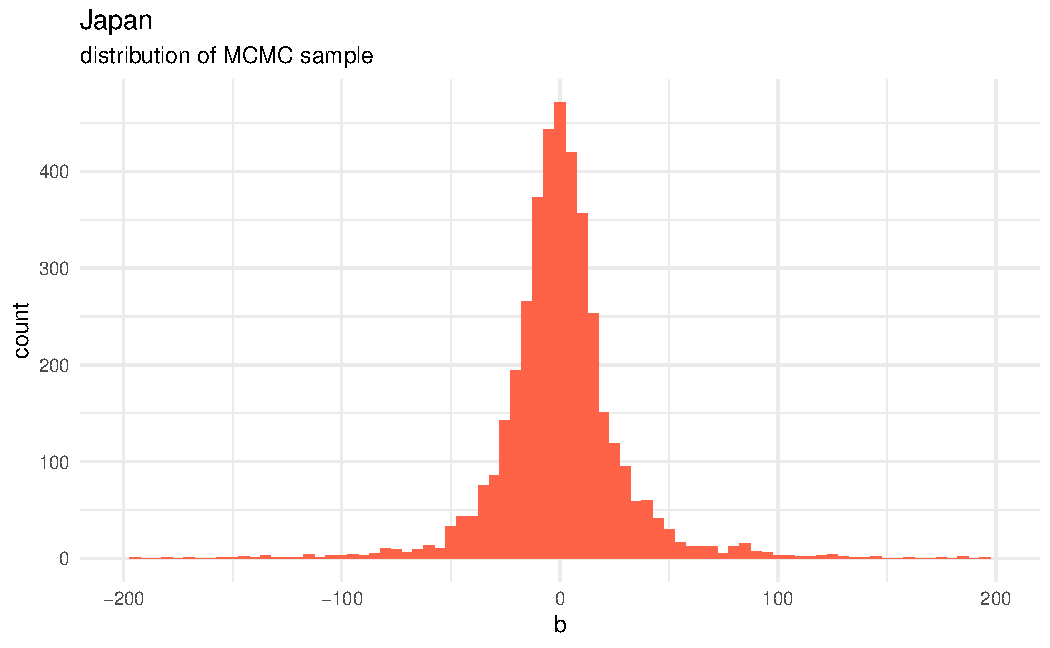
\includegraphics[width=12cm]{J_hist.pdf}
\caption{日本の$\beta$の分布}
\end{figure}

\begin{figure}[H]
\centering
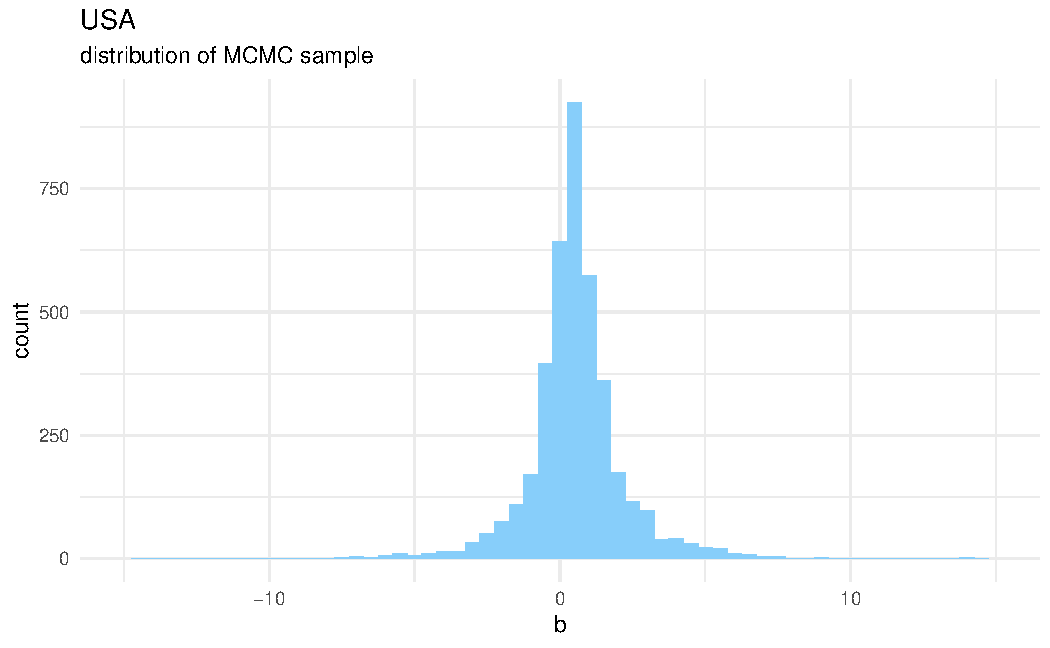
\includegraphics[width=12cm]{U_hist.pdf}
\caption{アメリカの$\beta$の分布}
\end{figure}
\end{document}
